\documentclass{article}

\usepackage{arxiv}

\usepackage[utf8]{inputenc} % allow utf-8 input
\usepackage[T1]{fontenc}    % use 8-bit T1 fonts
\usepackage{hyperref}       % hyperlinks
\usepackage{url}            % simple URL typesetting
\usepackage{booktabs}       % professional-quality tables
\usepackage{amsfonts}       % blackboard math symbols
\usepackage{nicefrac}       % compact symbols for 1/2, etc.
\usepackage{microtype}      % microtypography
\usepackage{lipsum}		% Can be removed after putting your text content
\usepackage{graphicx}
\graphicspath{ {./images/} }
\usepackage[square,numbers]{natbib}
\usepackage{doi}

\title{ZPY: Open Source Synthetic Data for Computer Vision}

\author{
	{\hspace{1mm}Hugo Ponte}\thanks{correspondence author} \\ 
	Zumo Labs \\
	\texttt{hugo@zumolabs.ai} \\
	\And
	{\hspace{1mm}Norman Ponte} \\
	Zumo Labs \\
	\texttt{norman@zumolabs.ai} \\
	\And
	{\hspace{1mm}Sammie Crowder} \\
	Zumo Labs \\
	\texttt{sammie@zumolabs.ai} \\
	\And
	{\hspace{1mm}Kory Stiger} \\
	Zumo Labs \\
	\texttt{kory@zumolabs.ai} \\
	\And
	{\hspace{1mm}Steven Pecht} \\
	Zumo Labs \\
	\texttt{steven@zumolabs.ai} \\
	\And
	{\hspace{1mm}Michael Stewart} \\
	Zumo Labs \\
	\texttt{michael@zumolabs.ai} \\
	\And
	{\hspace{1mm}Elena Ponte} \\
	Zumo Labs \\
	\texttt{elena@zumolabs.ai} \\
}

% Uncomment to remove the date
\date{}

\renewcommand{\headeright}{Technical Report}
\renewcommand{\undertitle}{Technical Report}

% PDF metadata
\hypersetup{
pdftitle={ZPY: Open Source Synthetic Data for Computer Vision},
pdfsubject={cs.CV},
pdfauthor={Hugo Ponte, Norman Ponte, Sammie Crowder, Kory Stiger, Steven Pecht, Elena Ponte},
pdfkeywords={Computer Vision, Synthetic Data, Machine Learning, Open Source, Python, Blender},
}

\begin{document}
\maketitle

\begin{abstract}
Synthetic data presents a unique solution to the huge data requirements of computer vision with deep learning. In this work, we present zpy \footnote{All code is available on GitHub at \url{http://github.com/ZumoLabs/zpy}}, an open source framework for creating synthetic data. Built on top of Blender, and designed with modularity and readability in mind.
\end{abstract}

\keywords{Computer Vision \and Synthetic Data \and Machine Learning \and Open Source \and Python \and Blender}

% https://www.overleaf.com/learn/latex/Inserting_Images
\begin{figure}[!ht]
	\centering
	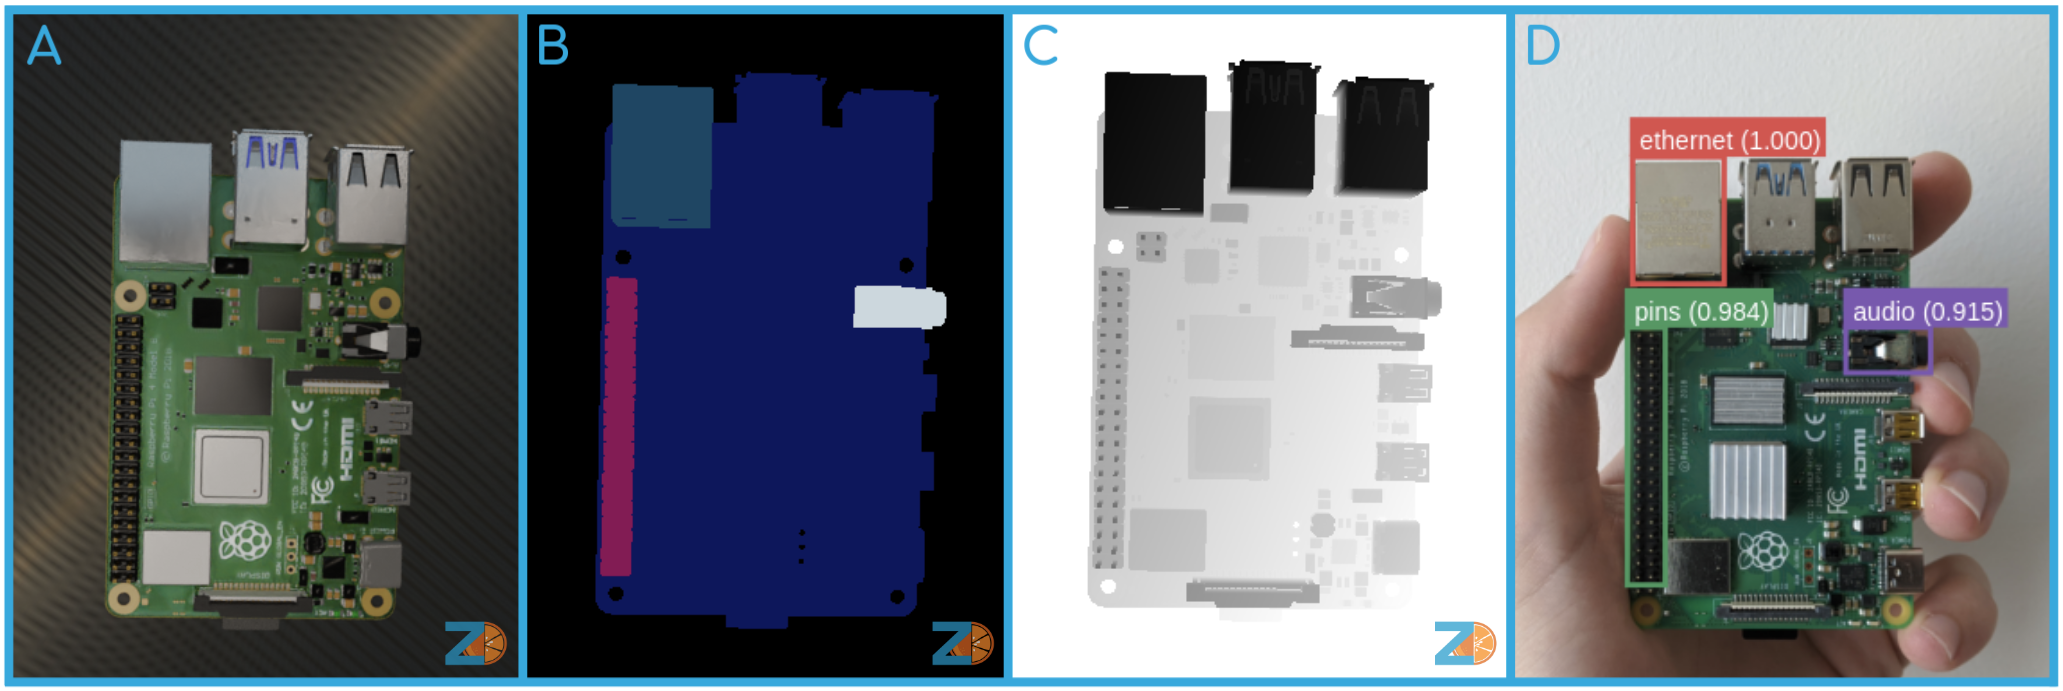
\includegraphics[width=\textwidth]{cover.png}
	\caption{Synthetic images of a raspberri pi created with zpy: (A) color image, (B) segmentation image, (C) depth image, (D) prediction image}
	\label{fig:fig1}
\end{figure}

\section{Introduction}
\label{sec:introduction}

Open source machine learning frameworks (references)

Deep learning has exploded in popularity due to large open source frameworks such as tensorflow and pytorch
What is synthetic data (references)

Challenges with synthetic data

Sim2Real Gap and domain randomization

Black box nature of ML

\section{Background}
\label{sec:background}

\subsection{3D}
\label{sec:3d}

3D, short for the three dimensions of space we experience, is a catch-all term used to describe the varied technologies used to create virtual worlds. The technology stack for 3D can be roughly split into two broad categories \emph{asset creation} and \emph{asset scripting}. Asset creation \ref{sec:assetcreation} is the process of creating virtual objects, scenes, and materials. Asset scripting \ref{sec:assetscripting} is the process of controlling those assets and their behavior over time. Both of these technologies require human expertise and artistic talent \ref{sec:humanexpertise}.
 
\subsubsection{Asset Creation}
\label{sec:assetcreation}

Assets are digital representations of a 3D object. In the engineering and manufacturing world, assets are created using computer aided design (CAD) software such as AutoCAD \citep{autocad}, Solidworks \citep{solidworks}, Onshape \citep{onshape}, and Rhino \citep{rhino}. In the entertainment industry, assets are created using modeling software such as Maya \citep{maya}, 3DSMax \citep{3dsmax}, and Cinema4D \citep{cinema4d}. Modeling and CAD are two different words for the same thing: deciding the connectivity and placement of a graph of points, also called vertices, which define the boundaries of an object. Vertices are connected by edges, and a closed loop creates a polygon known as a face. Many 3D assets can be organized into scenes, which may contain other unique virtual objects such as simulated lights and cameras. Finally, asset creation also encompasses teh process of material creation. The appearance of a virtual object is determined by a material, which may define rules for the reflectivity, specularity, and metallic-ness of the object as a function of lighting conditions.

\subsubsection{Asset Scripting}
\label{sec:assetscripting}

There is a fourth dimmension to our reality which is time. Asset scripting is the process of defining the behavior of assets and scenes over the dimmension of time. One such process is called animation, which consists of an expert human artist pupeteering and deforming a mesh frame by frame to create the illusion of natural movement. Specialized software is often used to automate this task as much as possible, and technologies such as Motion Capture (MoCap) are often used to record the movement of real objects and play those movements back on virtual assets.

Game Engines are software tools which allow for manipulation of assets in a more structured and systematic way by providing software interfaces to control the virtual world. Used extensively in the video game industry after which they were named, examples include Unity \citep{unity3d}, Unreal Engine \citep{unrealengine}, GoDot \citep{godot}, and Roblox \citep{roblox}. These game engines allow for rule-based spawning, animation, and complex interactions between assets in the virtual world.

\subsubsection{Human Expertise}
\label{sec:humanexpertise}

Houdini \citep{houdini} and Blender \citep{blender}

\subsection{Deep Learning}
\label{sec:deeplearning}

Modern deep learning can be implemented in a variety of programming languages including Python, R, Julia, Scala, Ruby, Octave, MATLAB, and even C/C++. Amongst these, Python has emerged as the lingua franca, rising to the top in part due to the popularity of open source frameworks such as TensorFlow \citep{tensorflow}, PyTorch \citep{pytorch}, and Scikit-Learn \citep{scikit-learn}.

\subsection{Synthetic Data}
\label{sec:syntheticdata}

The synthetic data workflow can be broadly divided into three categories: simulation design, generation, and tuning.

BlenderProc, Synthesis, LexSet

\section{Motivation}
\label{sec:motivation}

\subsection{Democratization of Data}

The datasets used by companies today are almost exclusively collected.

Data for ML systems is collected. Only companies that have the scale and have set up the infrastructure to collect and store large datasets will have the datasets required to train models.

A huge market for the selling and reselling of collected data has emerged, which presents an existential threat to privacy.

The high cost of data labeling makes it unavailable to those without huge resources

\subsection{Fairness and Bias}

The real world is biased and unfair.

ML systems trained on this data will reflect the same bias during inference.

\begin{figure}
	\centering
	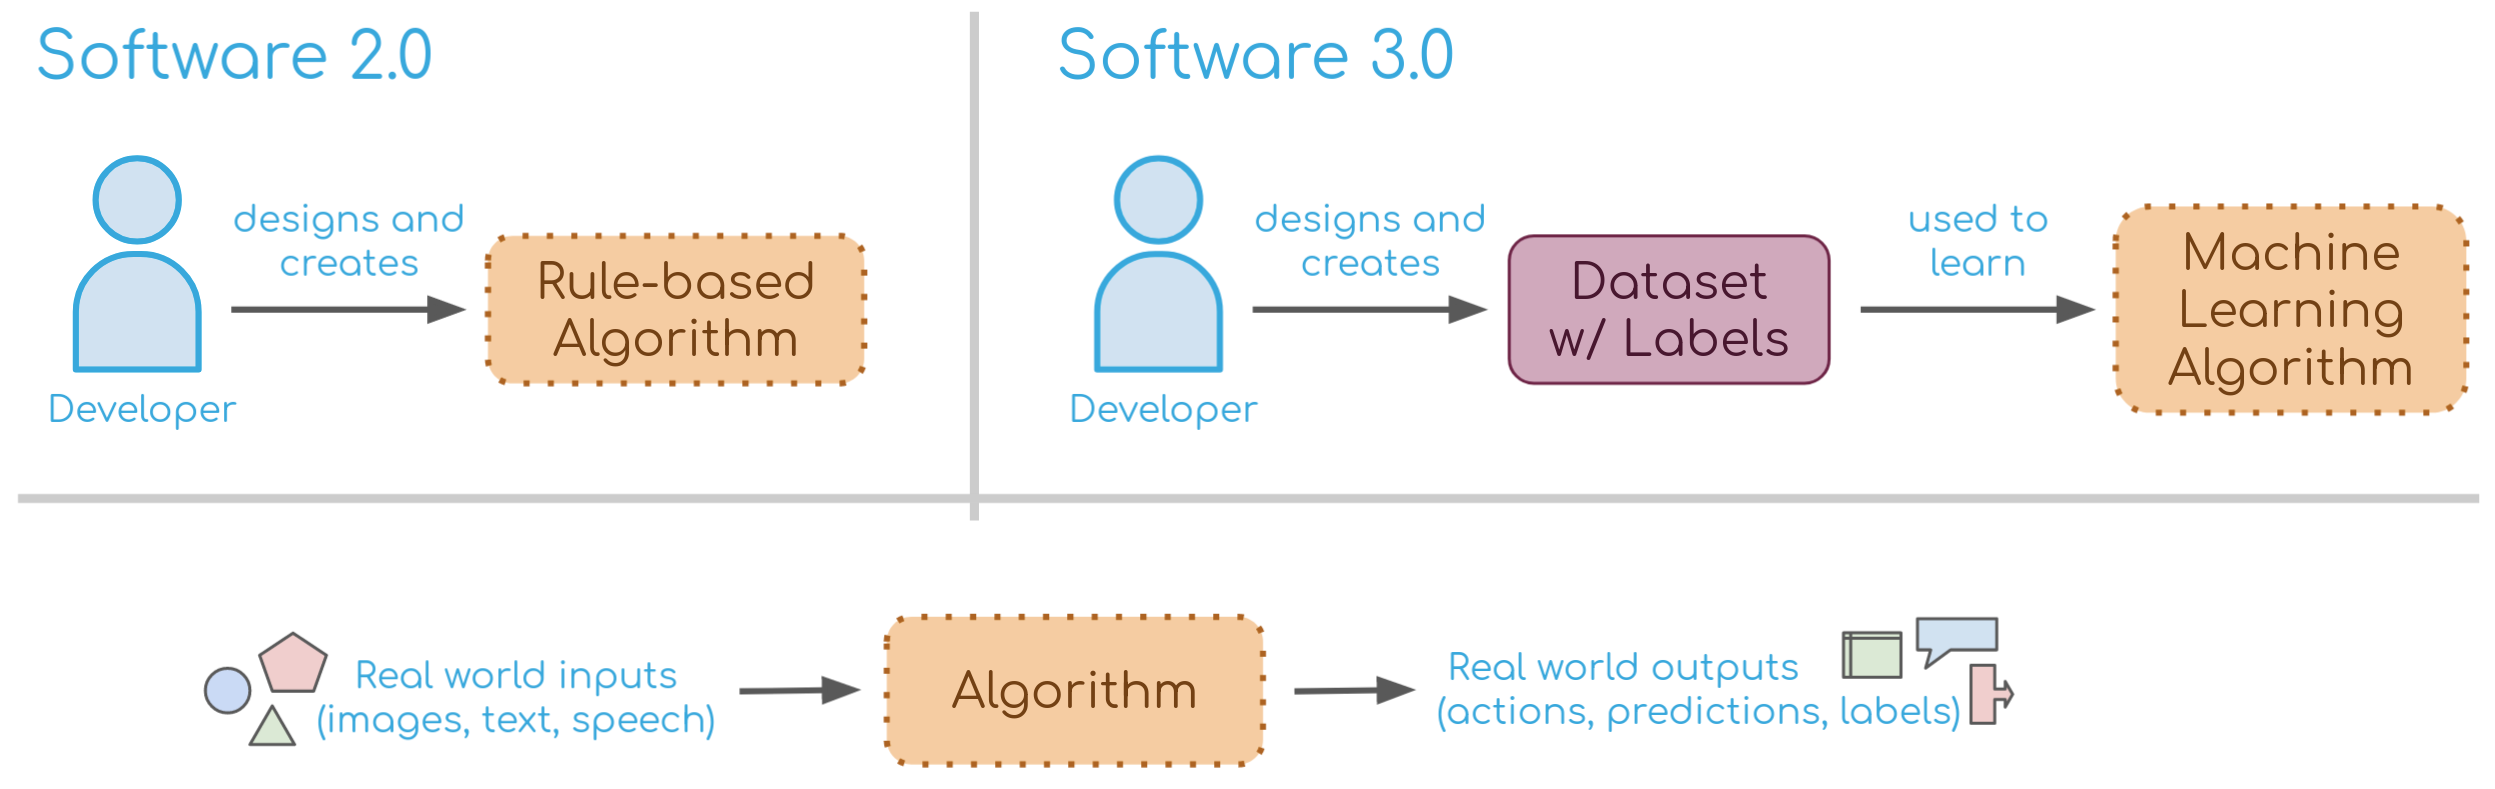
\includegraphics[width=\textwidth]{software3.png}
	\caption{Software 3.0: the developer transitions from writing explicit algorithms to creating and curating datasets which are used to train machine learning models.}
	\label{fig:fig2}
\end{figure}

\subsection{Software 3.0}
\label{sec:software3.0}

Data creation as a new paradigm for “programming”.

In the software world today, developers write explicit sets of rules (known as algorithms). These algorithms are then deployed into production systems, which consume input data and output actions.

In the software of tomorrow, developers will curate a dataset which will be used to train a deep learning model. This model will then be deployed into a production system, which will consume input data and output actions. This changes the workflow of developers from explicitly writing rules to instead creating the datasets which are then parsed to create algorithms.

\section{Project Features}
\label{sec:projectfeatures}

TODO

\subsection{Blender Addon}
\label{sec:blenderaddon}

As explained in section X, deep learning is a python-first discipline. If we wish to include deep learning practitioners in the 3D stack it is thus of critical importance that we provide a python interface for the 3D workflow.

\subsection{Cloud Backend}
\label{sec:cloudbackend}

Computing has traditionally relied on Moore’s Law to increase the power of individual computers. In the past decade the individual compute power of a single computer has not increased significantly, and instead the ability to coordinate a large number of individual computers on a single task has become the method for increasing computation. This type of parallel computing has been democratized through the availability of cloud computing platforms such as AWS, GCP, and Azure. However, these platforms remain difficult for the average developer to use effectively, and domain experts are usually required to take software running on a single computer and scale it across many computers in parallel.

Abstracting away the difficulties of the cloud workflow and providing an intuitive and convenient interface for parallelizing computation is thus important for the democratization of deep learning and synthetic data workflows. Much like platforms have emerged for the training and tuning workflows of deep learning, an opportunity exists to create platforms for the generation and tuning workflows of synthetic data.


\subsection{User Interfaces}
\label{sec:cloudbackend}

We provide three different interfaces to interact with our product: an API, a CLI, and a graphical WebApp.

Power users want an API (application programming interface) and CLI (command line interface).

Building a ramp for the bulk of the developer community requires a GUI

\section{Design}
\label{sec:design}

Hidden complexity

When designing software systems, there is usually a tradeoff between flexibility and simplicity. Simplicity is the ability to perform a task with minimal amount of work and a limited understanding of the software package. Flexibility is the ability to support many different tasks and allow for customization.

Random hdri and textures use default random textures unless a specific path is given

Pythonic syntax

One of the core features of Python is the language’s human readable syntax. Python does not enforce function and variable type annotations, which makes it quicker to prototype code.

Functions in zpy are flexible in the arguments that they accept. The `zpy.opject.segment()` function call can accept an object directly of type `bpy.types.Object`, but it will also accept the unique string name of that object. 

Extensibility

Zpy modules are separated by dependencies

Zpy modules are independent of each other, a monolithic system is much harder to update and maintain


\begin{figure}
	\centering
	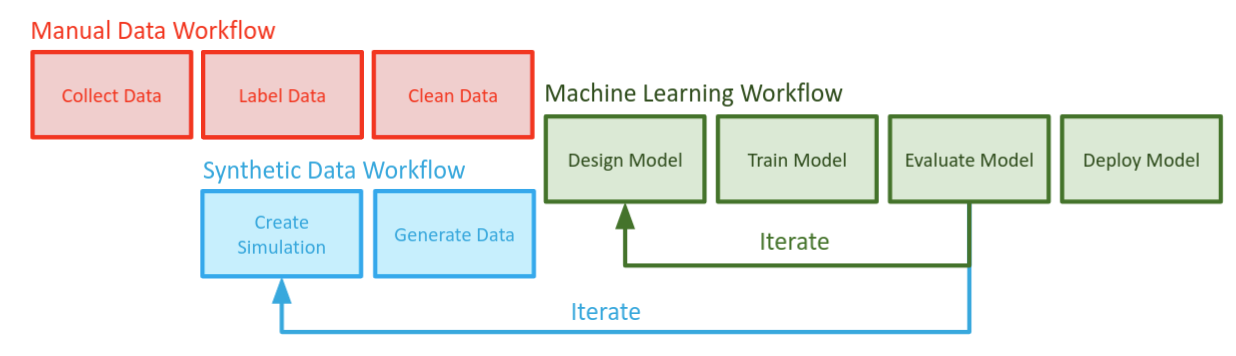
\includegraphics[width=\textwidth]{workflow.png}
	\caption{The Synthetic Data Workflow allows for iteration of the dataset.}
	\label{fig:fig3}
\end{figure}

\section{Workflow}
\label{sec:workflow}

See Figure \ref{fig:fig3}.

The full workflow for synthetic data can be reduced into four key steps:

\begin{itemize}
	\item \emph{Design}.
	\item \emph{Generation}.
	\item \emph{Evaluation}.
	\item \emph{Iteration}.
\end{itemize}

\subsection{Design}
\label{sec:worflowdesign}

Design the Sim

Sim is short for simulation.

A sim is controlled through a single run script, which has a single run() function

Relevant parameters are put as kwargs in the run() function, which allows configuration through gin config

Gin configuration allows for modular python library design

\subsection{Generation}
\label{sec:generation}

Generate the dataset

Datasets are rendered frame by frame. Separate rendering passes are required for segmentation and color images.

Cycles vs Eevee

\subsection{Evaluation}
\label{sec:evaluation}

Evaluate the datasets

Sweeping over dataset hyperparameters (much like sweeping over model architecture parameters)

Fine-tuning pre-trained models as a proxy for dataset performance

\subsection{Iteration}
\label{sec:iteration}

Iterate

Least understood part of developing with synthetic data

The promise of AutoML for datasets


\section{Example}
\label{sec:example}

Package detection

\begin{itemize}
	\item Background material and texture.
	\item Lighting intensity and positioning.
	\item Object material and texture.
	\item Number of objects in view.
\end{itemize}

\subsection{Domain Randomization}
\label{sec:domainrandomization}

Effect of domain randomized lighting

Effect of domain randomized backgrounds

\subsection{Training Curicculum}
\label{sec:curicculum}

Pre-training w/ real and fine-tuning on synthetic

Training only on synthetic

Training on mixed synthetic and real

\section{Conclusion}
\label{sec:conclusion}

TODO

\bibliographystyle{abbrvnat}
\bibliography{references}

\end{document}
